\section{Method}

\subsection{Study Design}

We conducted a two-phase qualitative household study in Bangladesh from January to June 2026. The study examined how older adults and family caregivers organized medication work within the household and how those arrangements shaped their experiences with a medication-support prototype. All study sessions took place in participants' homes and were conducted in Bangla.

\textbf{Phase 1} consisted of formative interviews, contextual observation, and medication-routine walkthroughs. We examined how medicines were stored and taken, how responsibilities were distributed among household members, how routines were disrupted, and how relatives participated in reminding, checking, purchasing, or otherwise supporting medication use. We conducted a formative analysis of Phase 1 before developing the prototype so that its design reflected practices documented in participating households.

We then developed and installed a medication-support prototype informed by the Phase 1 findings. Participants used the prototype for two weeks. The deployed system provided medication reminders and records, stated whom it was serving, and could ask whether a family member should be involved when a scheduled dose remained unconfirmed.

\textbf{Phase 2} consisted of post-deployment interviews conducted after the two-week deployment. These interviews examined participants' reported experiences with deployed features and their reasoning about several additional design mechanisms that had been specified but were not implemented. We distinguished these forms of evidence throughout the study: accounts of deployed features are treated as reported experiences of use, whereas responses to unimplemented mechanisms are treated as judgments about proposed designs.

We treated the household as the primary context of medication management because relatives often participated in purchasing medicines, reading labels, organizing doses, providing reminders, and checking whether scheduled doses had been taken \cite{106}. Where such coordination occurred, we recruited an involved family caregiver as a participant in their own right. When an older adult and caregiver described the same household event differently, we retained both accounts rather than reconciling them into a single version.

\subsection{Participants and Recruitment}

We recruited participants through snowball sampling, beginning with the research team's social networks and continuing through referrals from friends, colleagues, and community groups. Approximately 30 households were approached. Participation was voluntary and unpaid.

Older adults were eligible if they were at least 65 years old and took medication daily. Family members were eligible if they performed medication-related work for an older adult living in the same household.

The final sample comprised 25 participants: 17 older adults and eight family caregivers. Phase 1 included 16 older adults and eight caregivers, while Phase 2 included 17 older adults and seven caregivers. Sixteen older adults and seven caregivers participated in both phases; one older adult participated only in Phase 2, while one caregiver participated only in Phase 1.

Older adults were 65--80 years old (mean = 69.4; median = 68), including nine women and eight men. Eleven needed large text, including two who could not read, while nine described low or very low smartphone comfort. Five reported taking one medicine daily, three reported eight or more, and one reported thirteen medicines across three dose times.

The eight caregivers included four women and four men. Six reported their age, ranging from 20 to 31 years. Their relationships to the older adults included daughters, sons, a daughter-in-law, and grandchildren. Tables~\ref{tab:older-adults} and~\ref{tab:caregivers} report participant-level demographic, medication, device, and caregiving information.

\begin{table}[t]
  \caption{\textbf{Older adults taking daily medication (n = 17).}}
  \label{tab:older-adults}
  \small
  \begin{tabular}{lrlrrl}
    \toprule
    ID & Age & Gender & Daily medicines & Dose times/day & Deployment device \\
    \midrule
    P01 & 72 & M & 4 or more & 4 & Own smartphone \\
    P02 & 65 & M & 1 & 1 & Household smartphone \\
    P03 & 66 & F & 3 to 4 & 2 & Own smartphone \\
    P04 & 69 & M & 4 & 3 & Own smartphone \\
    P05 & 68 & F & 1 & 1 & Household smartphone \\
    P06 & 67 & M & 1 & 1 to 2 & Household smartphone \\
    P07 & 71 & F & 3 to 4 & 2 or more & Own smartphone \\
    P08 & 67 & F & 2 to 4 & 2 & Household smartphone \\
    P09 & 68 & F & 3 to 4 & 3 & Household smartphone \\
    P10 & 78 & M & 2 & 3 & Own smartphone \\
    P11 & 65 & M & 5 to 6 & 3 & Own smartphone \\
    P12 & 71 & F & 1 & 1 & Own smartphone \\
    P13 & 66 & F & 1 & 1 & Own smartphone \\
    P14 & 66 & F & 5 & Not recorded & Not recorded \\
    P15 & 80 & M & 8 to 10 & 3 & Not recorded \\
    P16 & 76 & F & 13 & 3 & Not recorded \\
    P17 & 65 & M & 8 & 2 & Own smartphone \\
    \bottomrule
  \end{tabular}
\end{table}

\begin{table}[t]
  \caption{\textbf{Family caregivers (n = 8).}}
  \label{tab:caregivers}
  \small
  \begin{tabular}{lrllll}
    \toprule
    ID & Age & Gender & Relation & Older adults supported & Daily medicines managed \\
    \midrule
    C01 & Not recorded & F & Daughter & Mother and father & 3 to 4, and 2 \\
    C02 & Not recorded & F & Daughter & Mother and grandfather & 2 or more, and 3 to 4 \\
    C03 & 21 & M & Son & Father and mother & 3 to 4, and 2 \\
    C04 & 31 & M & Son & Mother & 2 \\
    C05 & 20 & F & Daughter-in-law & Father-in-law and mother-in-law & 4 to 5 \\
    C06 & 22 & F & Granddaughter & Grandmother & 5 to 6 \\
    C07 & 25 & M & Grandson & Grandfather & 10 \\
    C08 & 25 & M & Grandson & Grandmother and mother & 5 to 6 \\
    \bottomrule
  \end{tabular}
\end{table}

\subsection{Phase 1: Formative Household Study}

Following prior situated-practice work \cite{61,9}, Phase 1 examined medication practices before participants encountered the prototype. We used separate semi-structured interview protocols for older adults and family caregivers; the complete protocols are provided in \textbf{Appendix A1} and \textbf{Appendix A2}, respectively.

The interviews covered daily medication routines, medicine storage, disruptions, recent missed or delayed doses, reading and interaction conditions, family involvement, responsibility sharing, technology use, and what happened when the person who usually provided support was unavailable. Rather than asking only about general preferences, we asked participants to reconstruct recent episodes and demonstrate relevant parts of their routines in the places where medication work occurred \cite{61,9}.

The caregiver protocol focused on caregivers' own medication-related work, including how responsibilities developed, how they checked whether medicines had been taken, and what happened when they were unavailable \cite{106}. We distinguished caregivers' accounts of their own activities from their interpretations of the older adult's experience and from jointly described household events.

Each session followed the same general sequence: consent, observation of the immediate setting, semi-structured interviewing, a medication-routine walkthrough, and a closing design reflection. With permission, sessions were audio-recorded in Bangla. Researchers also documented medicine storage, relevant lighting and noise conditions, medication-related artifacts, and household members involved during demonstrations.

Phase 1 supports claims about existing medication practices and the requirements that informed prototype development. It provides no evidence about prototype use.

\subsection{Formative Analysis and Prototype Development}

We conducted a formative analysis of the Phase 1 material before prototype development. The analysis identified requirements concerning timely reminders, medicine and timing information, reduced dependence on manually consulting a schedule, family awareness of unconfirmed doses, simplified interaction, readable presentation, and opportunities for family involvement. After Phase 2, the Phase 1 material was considered again as part of the full qualitative analysis described below.

\begin{figure}[t]
  \centering
  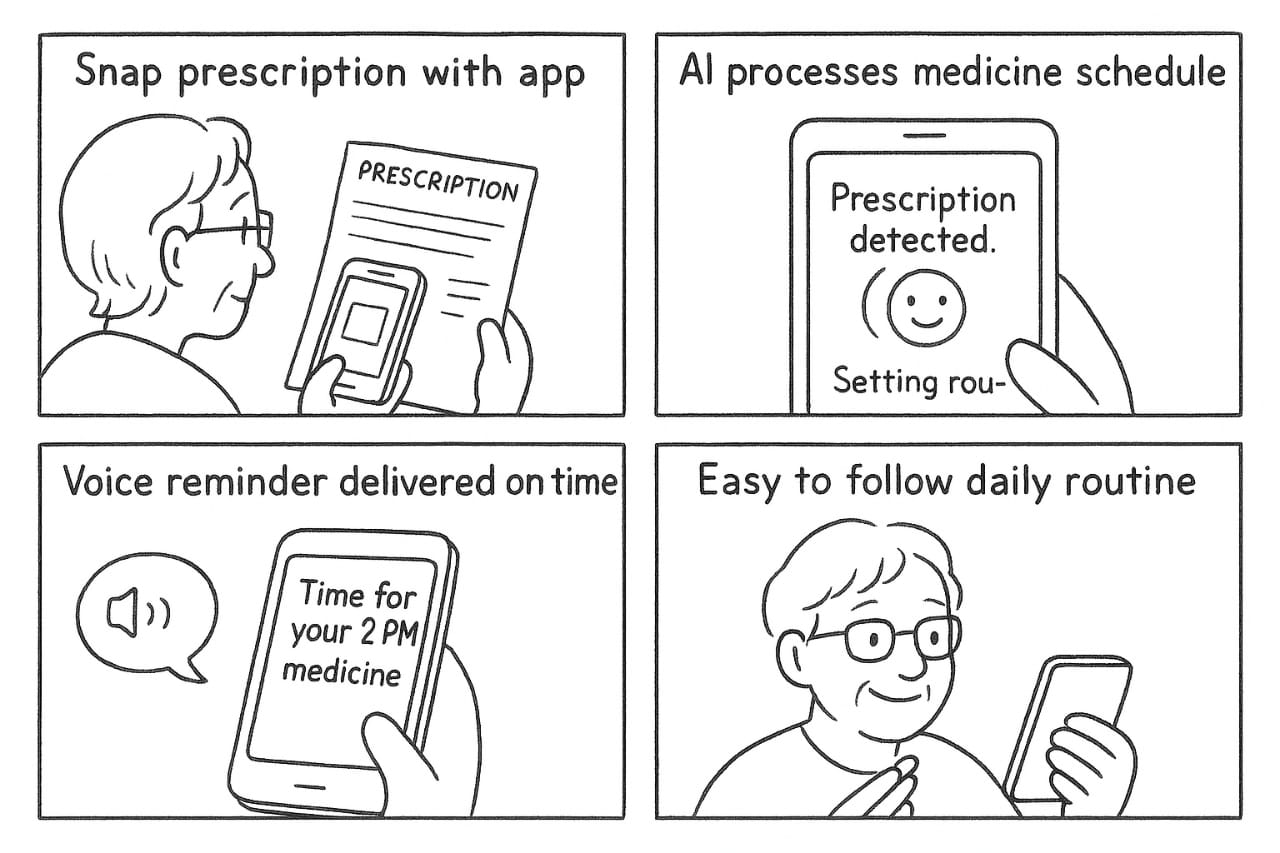
\includegraphics[width=\linewidth]{Figures/initial-uses.jpg}
  \Description{Four-panel storyboard of the design concept: capturing a prescription, the schedule being set from it, a spoken reminder at dose time, and a routine the person can follow.}
  \caption{Four-panel storyboard of the design concept: capturing a prescription, the schedule being set from it, a spoken reminder at dose time, and a routine the person can follow.}
  \label{fig:design-concept}
\end{figure}

Figure~\ref{fig:design-concept} shows how these requirements informed the initial design concept. The concept included prescription capture, schedule creation, spoken reminders, and a medication routine organized around those reminders. Prescription capture was specified in the concept but was not implemented in the deployed prototype.

Participants or family members therefore entered medication schedules manually. At scheduled times, the deployed prototype delivered reminders containing the medicine name and timing. Participants could confirm that a dose had been taken, which updated the medication logbook, streak, and daily heat map.

When a scheduled dose remained unconfirmed, the system could ask whether a family member should be notified. Participants could decline the request, and the family-notification path proceeded only after permission was granted. Medication schedules and changes in whom the system served remained under human control.

The streak and heat map were designed to make medication records visible within the household and create possible occasions for family response. This was a design rationale rather than an assumed effect of the system.

\begin{figure}[t]
  \centering
  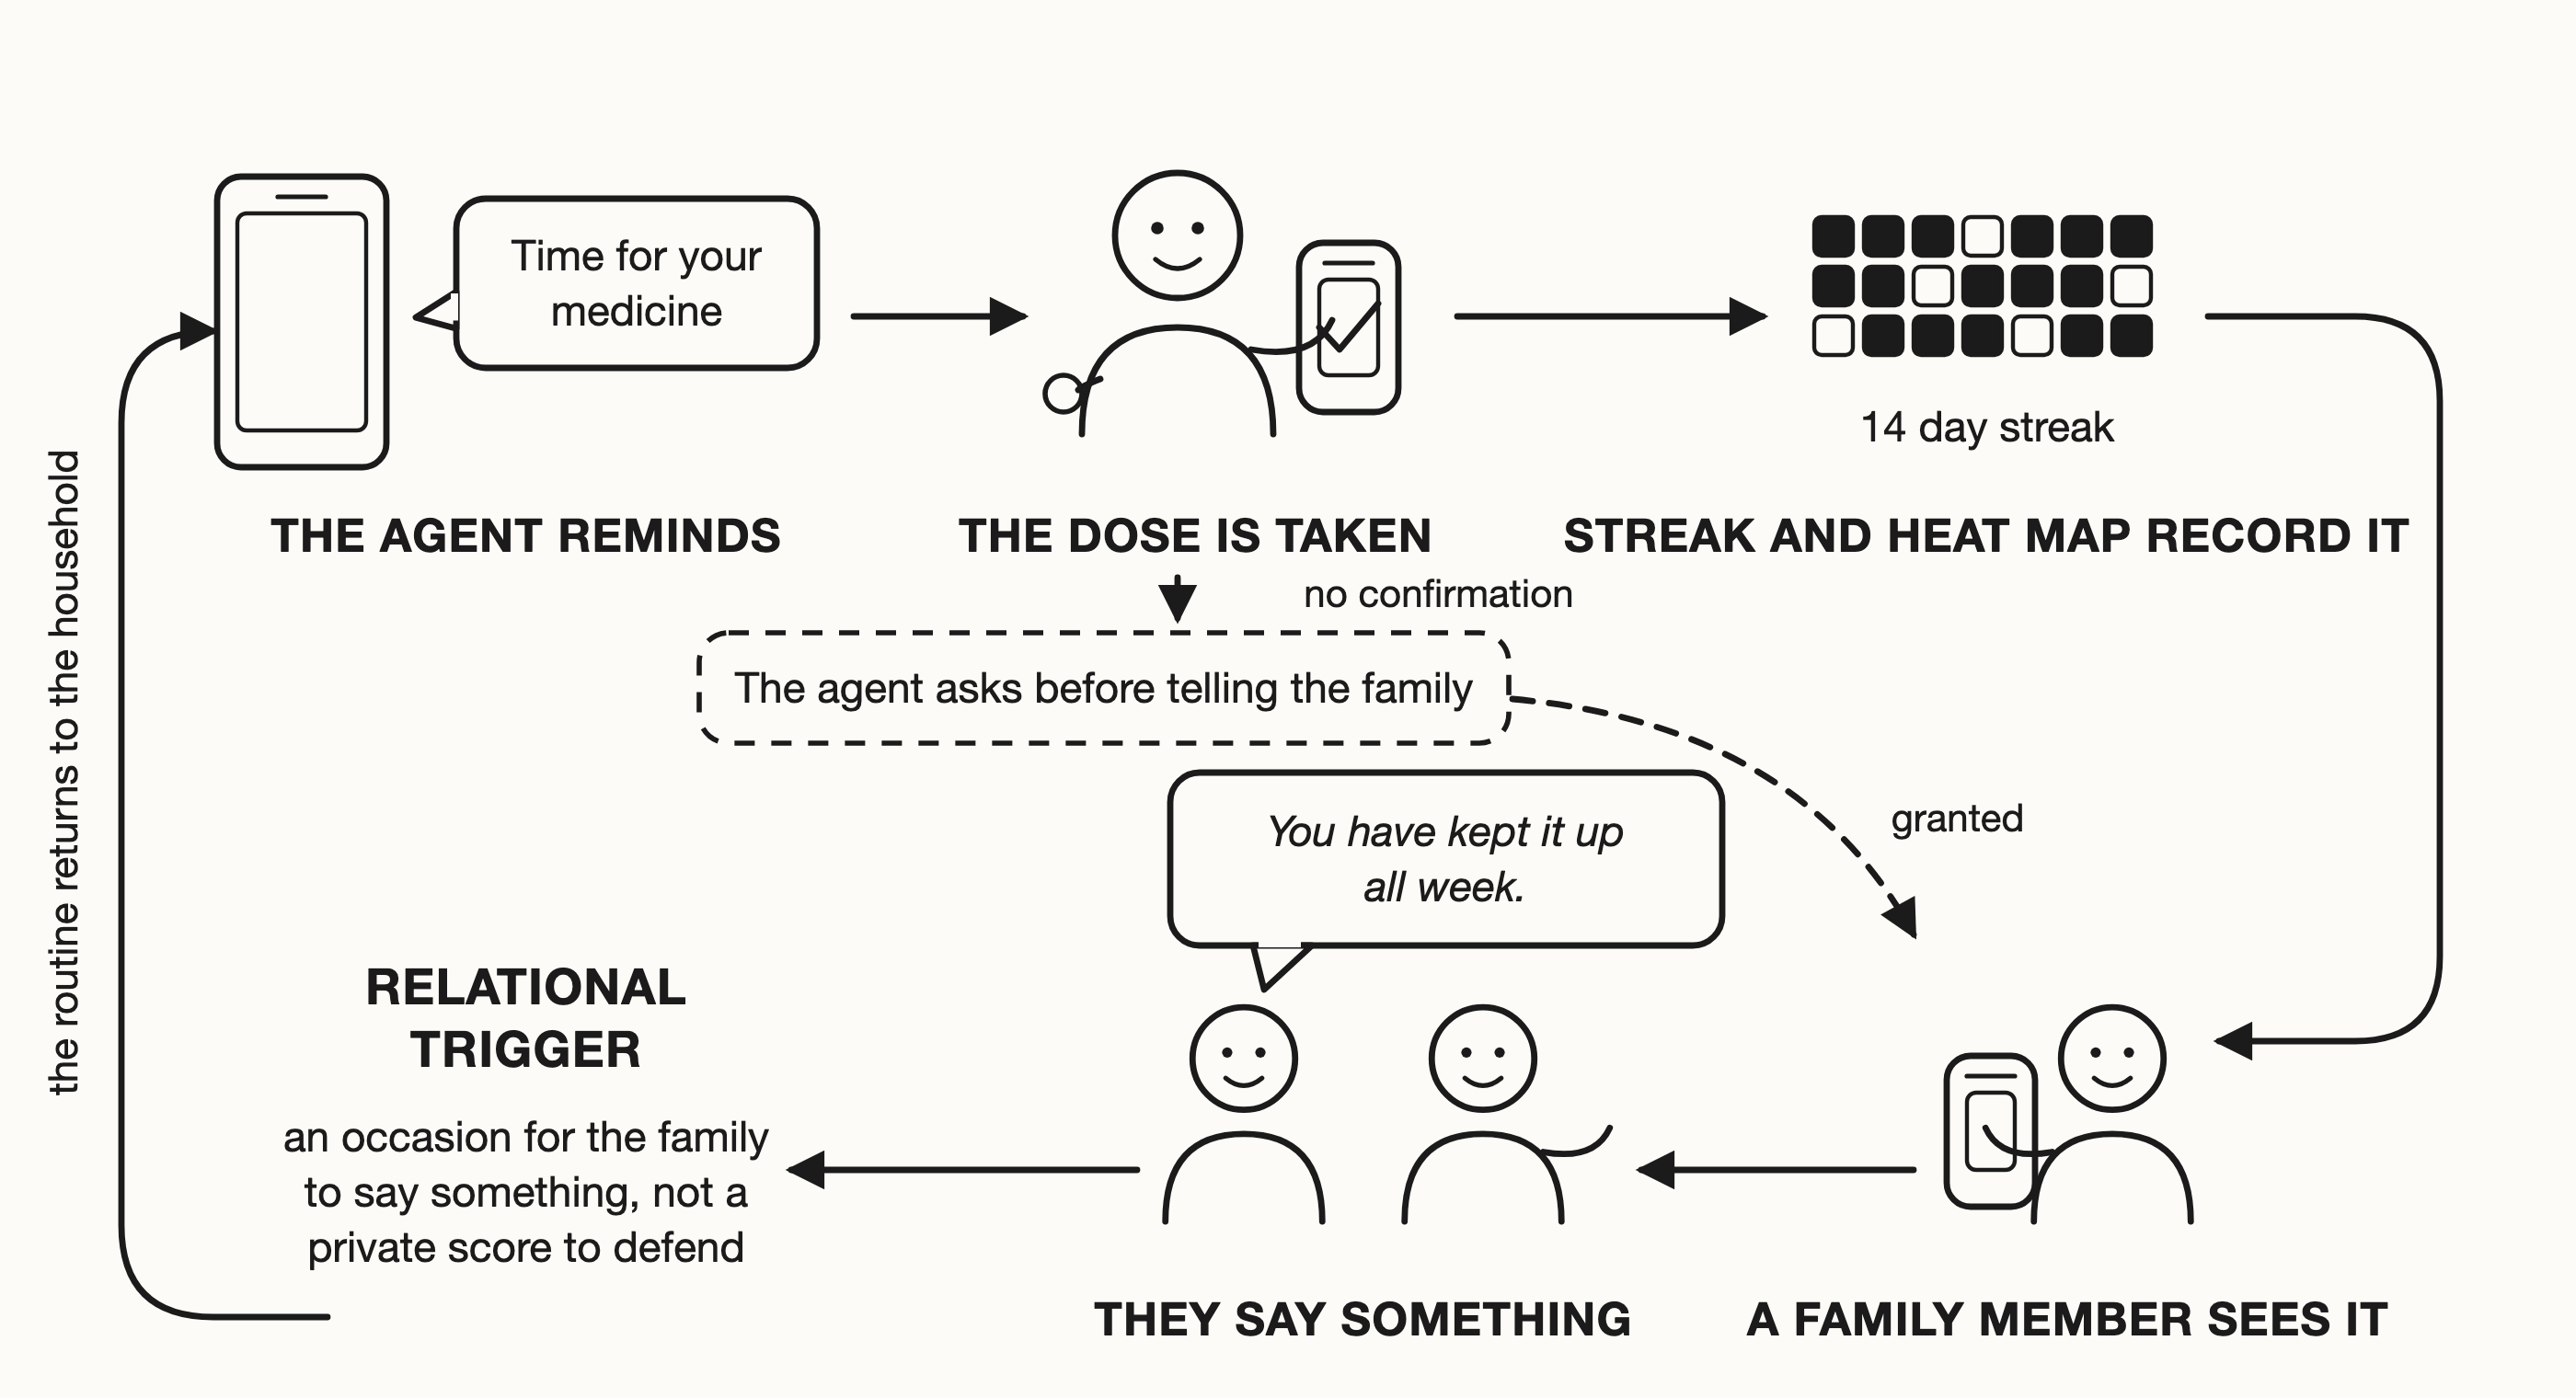
\includegraphics[width=\linewidth]{Figures/relational-trigger-loop.png}
  \Description{Loop diagram: the agent reminds, the dose is taken, a streak and heat map record it, a family member sees the record and says something, and the routine returns to the household. A dashed branch shows an unconfirmed dose reaching the family only after the agent asks and the older adult grants.}
  \caption{Loop diagram: the agent reminds, the dose is taken, a streak and heat map record it, a family member sees the record and says something, and the routine returns to the household. A dashed branch shows an unconfirmed dose reaching the family only after the agent asks and the older adult grants.}
  \label{fig:trigger-loop}
\end{figure}

Figure~\ref{fig:trigger-loop} presents the interaction loop implemented during deployment. After a scheduled reminder, an older adult could confirm taking the dose, which updated the medication record, streak, and heat map. When a dose remained unconfirmed, the family-notification path could proceed only after the participant granted permission.

Four mechanisms in the broader design specification were not implemented in the deployed version: a risk-graded weakening veto, patterned interpretation of silence, a probationary onboarding mode, and shared family scores. These mechanisms were discussed during Phase 2 as proposed designs rather than as features participants had used.

\subsection{Phase 2: Household Deployment and Post-Deployment Study}

\subsubsection{Prototype Deployment}

Researchers installed the prototype during a home visit and configured the initial medication schedule with the older adult or, where relevant, the family member operating the household device. Onboarding covered scheduled reminders, the logbook, and the spoken announcement identifying whom the system was serving.

Nine older adults used personal smartphones, while five used household smartphones shared with or operated by relatives. Device information was unavailable for three participants. We treated shared and intermediated operation as part of the deployment context rather than as equivalent to independent smartphone use, consistent with prior accounts from the region \cite{1,33,98}.

Participants used the prototype for two weeks before the Phase 2 interviews.

\subsubsection{Post-Deployment Interviews}

We returned to participating households after deployment and conducted post-deployment interviews in Bangla. We used separate semi-structured protocols for older adults and family caregivers; the complete protocols are provided in \textbf{Appendix B1} and \textbf{Appendix B2}, respectively. When an older adult and an enrolled caregiver both participated, each discussed the deployment period from their own perspective.

Questions about deployed features covered reminders, announcements of whom the system was serving, medication records, requests for family involvement, occasions when participants accepted or declined those requests, family notifications, and changes participants noticed in their medication routines or family involvement. Interviewers first invited participants to describe experiences in their own terms and then used follow-up probes to reconstruct specific episodes.

The interviews also presented the four mechanisms that were not implemented. These were introduced as hypothetical design possibilities rather than experiences participants were assumed to have had. Several probes described possible interpretations of these mechanisms, so we distinguished episodes or interpretations volunteered by participants from agreement expressed after a probe introduced a possible interpretation. Prompted agreement alone was treated as weaker evidence during analysis.

Accounts of deployed features support claims about participants' reported experiences during the two-week period. Responses to unimplemented mechanisms support only claims about how participants reasoned about the proposed designs.

\subsection{Data Analysis}

\subsubsection{Transcription and Translation}

The verified Bangla transcripts served as the primary analytic record. Automatic speech recognition produced preliminary Bangla transcripts, and machine translation produced initial English renderings, but neither automated output was treated as final. Two Bangla-fluent researchers verified each transcript against the corresponding audio and checked the English rendering against the verified Bangla source. Coding and interpretation were conducted using the Bangla records, and researchers returned to the original Bangla whenever kinship terms, honorifics, relational expressions, or other meanings were not adequately represented in English. Automated systems were used only to support preliminary transcription and translation, not coding, theme development, or interpretation.

\subsubsection{Reflexive Thematic Analysis}

We analysed material from both phases using reflexive thematic analysis \cite{15,16}. Coding began inductively and attended to participants' accounts of medication routines, family involvement, responsibility, technology use, and experiences with the prototype. We worked across semantic and latent levels where relevant and treated themes as researcher-constructed interpretations rather than entities that independently emerged from the data \cite{15,16}.

Analysis began with repeated reading and memoing. The two researchers who conducted the interviews developed preliminary codes and discussed interpretations iteratively with the supervising researcher. We did not calculate inter-rater reliability because coder agreement was not used as a criterion for theme validity within our reflexive approach \cite{16,93}. Researchers then grouped related codes into candidate themes and repeatedly examined them against the underlying transcripts. Themes were revised, combined, separated, or renamed as the analysis developed.

We retained older adults' and caregivers' accounts separately during analysis. When participants described the same household event differently, we treated those differences as part of the data rather than resolving them into a single household account. We maintained analytic memos, coding records, theme maps, and records of cases that complicated developing interpretations. When an interpretation depended on language not adequately represented in English, we returned to the verified Bangla transcript. We make no claim of thematic saturation.

\subsection{Ethical Considerations}

The study received approval from the Brac University Ethics Committee before data collection began. All study procedures followed the approved protocol.

Researchers explained the study purpose, procedures, voluntary nature of participation, audio recording, data use, and automated transcription and translation before obtaining informed consent. Study information was read aloud so participants who could not read received the same information. Consent was obtained individually, and separate permission was requested for audio recording. Caregivers consented independently from the older adults whose medication routines they might discuss.

Personal names were replaced with participant identifiers, and the identifier key was stored separately from the analytic corpus. Participants could discontinue participation at any point.

Three researchers conducted the study. Two conducted the interviews, transcript verification, and coding, while a third supervised the analysis. All three are fluent in Bangla and English. Recruitment began through the research team's social networks, which made some households more reachable than others \cite{75,103}. We therefore do not make population-level claims from the sample.

The two-week deployment supports accounts of participants' experiences during that period rather than longer-term use. We did not measure medication adherence, medication errors, or health outcomes and make no claims that the prototype changed them. Responses to unimplemented mechanisms are similarly limited to participants' judgments about described designs rather than observed use.
